\documentclass{article}

%%%%%%%%%%%%%%%%%%%%%%%%%%%%%%%%%%%%%%%%%%%%%%%%%%%%%%%%
% Packages
%%%%%%%%%%%%%%%%%%%%%%%%%%%%%%%%%%%%%%%%%%%%%%%%%%%%%%%%

%\usepackage[utf8]{inputenc} % for overleaf/PLM
\usepackage[latin1]{inputenc} % averil local
\usepackage[T1]{fontenc} % hyphenation
\usepackage{fullpage} % DO NOT USE IN BEAMER
\usepackage[british,UKenglish,USenglish,american]{babel}
%\usepackage{appendix}
\usepackage{amssymb,amsmath,amsthm,enumerate}
\usepackage{mathtools} % coloneqq
%\usepackage{easybmat}
\usepackage{enumitem}
%\usepackage{tikz}
%\usepackage{caption}
\usepackage{float} % [H]
%\usepackage{bbold}
\usepackage{xcolor}
\usepackage{stmaryrd} % ll/rr brackets
%\usepackage[notcite, notref]{showkeys}
%\usepackage[tworuled,vlined,nofillcomment]{algorithm2e}
\usepackage[ruled,vlined]{algorithm2e}
%\usepackage{cases} % numbered lines in cases (numcases and subnumcases)
\usepackage[overload]{empheq} % source : https://tex.stackexchange.com/questions/31951/separate-labels-in-cases
\usepackage{cleveref} % \cref. 

%%%%%%%%%%%%%%%%%%%%%%%%%%%%%%%%%%%%%%%%%%%%%%%%%%%%%%%%
% Format
%%%%%%%%%%%%%%%%%%%%%%%%%%%%%%%%%%%%%%%%%%%%%%%%%%%%%%%%

\title{Numerical methods for plasma sheaths}
\author{
	Valentin Ayot\footnote{Institut de Math�matiques, CNRS, UMR 5251, Universit� de Bordeaux, F-33405 Talence, France. \texttt{valentin.ayot@u-bordeaux.fr}}, 
	 \ Averil Prost\footnote{INSA de Rouen, LMI (EA 3226 - FR CNRS 3335), 685 Avenue de l'Universit�, 76801 St Etienne du Rouvray cedex, France. \texttt{averil.prost@insa-rouen.fr}}, 
	 \ Christian Tayou-Fotso\footnote{Labo. J. A. Dieudonn�, UMR 6621, Universit� Nice-Sophia Antipolis, Parc Valrose, F-06108 Nice cedex 02, France. \texttt{christian.tayou-fotso@unice.fr}}.
 } 
\date{}

\SetKwRepeat{Do}{do}{while} % for algorithm2e package, add do-while

% set dashes instead of bullets for item lists
\setlist[itemize,1]{label=$-$}
\setlist[itemize,2]{label=$-$}
\setlist[itemize,3]{label=$-$}

% remove unnecessary formatting of clever references
\crefdefaultlabelformat{(#2#1#3)}
\crefname{equation}{}{}

%%%%%%%%%%%%%%%%%%%%%%%%%%%%%%%%%%%%%%%%%%%%%%%%%%%%%%%%
% Theorems
%%%%%%%%%%%%%%%%%%%%%%%%%%%%%%%%%%%%%%%%%%%%%%%%%%%%%%%%

\newtheorem{proposition}{Proposition}[section]
\newtheorem{definition}{Definition}[section]
\newtheorem{theoreme}{Theorem}[section]
\newtheorem{remarque}{Remark}[section]
\newtheorem{lemme}{Lemma}[section]
\numberwithin{equation}{section}

%%%%%%%%%%%%%%%%%%%%%%%%%%%%%%%%%%%%%%%%%%%%%%%%%%%%%%%%
% Commands
%%%%%%%%%%%%%%%%%%%%%%%%%%%%%%%%%%%%%%%%%%%%%%%%%%%%%%%%

\newcommand{\N}{\mathbb{N}}
\newcommand{\Z}{\mathbb{Z}}
\newcommand{\R}{\mathbb{R}}
\newcommand{\lp}{\left(}
\newcommand{\rp}{\right)}
\newcommand{\tran}[1]{\prescript{t}{}{#1}}
\newcommand{\vol}{\textup{Vol}}
\newcommand{\red}{\textcolor{red}}
\newcommand{\blue}{\textcolor{blue}}

\newcommand{\todo}[1]{{\color{red}\textbf{#1}}}
\newcommand{\vv}[1]{\begin{pmatrix} #1 \end{pmatrix}} % vector
\newcommand{\mysubeq}[2]{ % first argument : label, second : align content
	\begin{subequations}\label{#1}
		\begin{align}[left = {\empheqlbrace}]
			#2
		\end{align}
	\end{subequations}	
}

%\renewcommand\appendixpagename{Appendix}
%\renewcommand\appendixtocname{Appendix}
\renewcommand{\qedsymbol}{$\blacksquare$}

%%%%%%%%%%%%%%%%%%%%%%%%%%%%%%%%%%%%%%%%%%%%%%%%%%%%%%%%
%%%%%%%%%%%%%%%%%%%%%%%%%%%%%%%%%%%%%%%%%%%%%%%%%%%%%%%%
%%%%%%%%%%%%%%%%%%%%%%%%%%%%%%%%%%%%%%%%%%%%%%%%%%%%%%%%

\begin{document}
	
\maketitle

\begin{abstract}
This article is a report of the project achieved during the CEMRACS 2022.
\end{abstract}

%% Plan
% 1 : Model : 
% 	- motivation, model, difficulties
%	- boundary conditions
%	- symmetries
% 2 : Numerical methods
% 3 : Numerical results : DO WE HAVE SHEATHS????

\section{Plasma sheaths}

% What is a plasma - electrons and ions

Plasma sheaths draw interest since the observations of Irvin Langmuir in 1923. The physical phenomenon happens, for instance, when a metallic wall is in contact with a plasma. Both species will be absorbed by the wall, but with a rate proportional to their speed. Since the electrons are moving several order of magnitude faster than the ions, a positively charged layer (the \emph{Debye sheath}) forms near the boundary. 

\todo{Difficulties}

The purpose of this work is to investigate numerically the formation of this sheath. \todo{Work on biblio!} It follows previous work of \todo{ref travail Michel et Yann} on a periodic case, and of \todo{ref Mehdi, Ana�s} on a collisional model. Our aim is to study an ionization model with nonperiodic boundary conditions. The first section introduces the corresponding system, and derives the boundary conditions. The second section presents the numerical methods used to simulate the evolution of the plasma, and the third section gives some results and comparisons.

\paragraph{The model}

Let $t\in\mathbb{R}^+$ denote the time variable, $x\in [-1,1]$ denote the spatial variable in a normalized one-dimensional domain, and $v\in\mathbb{R}$ denote the speed variable. The distribution of species is described through their density in the phase space, denoted by $f_i : (t,x,v) \in \R^+ \times [-1,1]\times \R \mapsto \R$ for the ions, and $f_e : (t,x,v) \in \R^+ \times [-1,1]\times \R \mapsto \R$ for the electrons. To these kinetic quantities, we add the spatial densities $n_{i,e}$ and currents $J_{i,e}$, defined by
\begin{align}\label{eq:def_ni_ne}
	n_{i,e} (t,x) \coloneqq \int_{v\in\R} f_{i,e} (t,x,v) dv, \quad\text{and}\quad J_{i,e} (t,x) \coloneqq \int_{v\in\R} v f_{i,e} (t,x,v) dv. 
\end{align}
In the sequel, we will denote $n (t,x) \coloneqq n_i (t,x) - n_e(t,x)$, and $J(t,x) \coloneqq J_i(t,x) - J_e(t,x)$.

The evolution of the densities is modelled by the Vlasov-Poisson equations. Let $\varphi : \R^+ \times [-1,1] \mapsto \R$ denote the electric potential. Then
\mysubeq{eq:unsta_model}{
	\partial_t f_i + v \partial_x f_i - \partial_x \varphi \, \partial_v f_i &= \nu f_e && (t,x,v) \in \R_{*}^{+} \times ]-1,1[ \times \R, \label{eq:unsta_model_fi} \\
	\partial_t f_i + v \partial_x f_e + \frac{\partial_x \varphi }{\mu}\, \partial_v f_e &= 0 \quad\quad && (t,x,v) \in \R_{*}^{+} \times ]-1,1[ \times \R, \label{eq:unsta_model_fe} \\
	- \lambda^2 \partial^2_{xx} \varphi &= n (t,x) && (t,x) \in \R^{+} \times ]-1,1[. \label{eq:unsta_model_phi}
}
The physical parameters $\nu$, $\mu$ and $\lambda$ have the following meaning:
\begin{itemize}
\item $\nu \geqslant 0$ is the ionization frequency. It describes the rate of \todo{creation / production / injection ?} of ions in presence of electrons.
\item $\mu \coloneqq m_e / m_i$ is the mass ratio between electrons and ions.
\item $\lambda > 0$ is the Debye length.
\end{itemize}

In the sequel, we may use the electric field $E(t,x) \coloneqq - \partial_x \varphi(t,x)$ in place of the potential. The, the second-order Poisson equation rewrites as 
\begin{align}
	\lambda^2 \partial_x E (t,x) = n(t,x) \quad \quad (t,x) \in \R^{+} \times ]-1,1[. \label{eq:unsta_model_E}
\end{align}

\begin{remarque}
	To reduce the notations, we will use $f_s$, $s\in\{i,e\}$ to denote both the electronic and ionic distributions. The advection equations \cref{eq:unsta_model_fi,eq:unsta_model_fe} rewrite 
	\begin{align*}
		\partial f_s + v \partial_x f_s - c_s \partial_x \varphi \partial_v f_s = S_s,
	\end{align*}
	with the speed coefficients $c_s$ and source terms $S_s$ defined as
	\begin{align*}
		c_i \coloneqq 1, \quad c_e \coloneqq -\frac{1}{\mu}, \quad S_i \coloneqq \nu f_e, \quad S_e \coloneqq 0.
	\end{align*}
\end{remarque}

The densities $f_i$ and $f_e$ are subject to initial and boundary conditions, given by
\mysubeq{eq:unsta_model}{
	f_{s}(0,x,v) &\coloneqq f_{s}^0(x,v) && (x,v) \in ]-1,1[ \times \R, \label{eq:init} \\
	f_{s}(t,x=\pm 1,\pm v < 0) &\coloneqq 0  && t \in \R^+_*. \label{eq:fie_bc}
}
The homogeneous boundary condition \cref{eq:fie_bc} stems from the non-emitting wall model: the boundary absorbs particles without any reflection.

To completely describe the model, we still need to provide boundary conditions for the Poisson problem \cref{eq:unsta_model_phi}. A first one is given by the choice of a reference potential
\begin{align}
	\varphi(t,0) = 0 \quad \quad \forall t \in \R^+. \label{eq:phi_nul_0}
\end{align}
To derive a second boundary condition, we introduce a fundamental symmetry assumption.

\paragraph{Symmetry}

We will look for \emph{symmetric solutions} satisfying 
\begin{align}\label{eq:phi_is_pair}
	\varphi(t,x) = \varphi (t,-x) \quad \quad (t,x) \in \R^+ \times [-1,1].
\end{align}
By derivation with respect to $x \in ]-1,1[$, we immediatly obtain 
\begin{align*}
	\partial_x \varphi(t,x) = - \partial_x \varphi (t,-x), \quad \text{i.e.} \quad E(t,x) = - E(t,-x).
\end{align*}
In particular, the electric field vanishes at $x=0$, and the Neumann boundary condition
\begin{align}\label{eq:phi_bc_neumann}
	\partial_x \varphi (t,0) = 0 \quad \text{or equivalently} \quad E(t,0) = 0
\end{align}
may be used (with \cref{eq:phi_nul_0}) to close the Poisson equation \cref{eq:unsta_model_phi}.


Let us notice that the advection equations \cref{eq:unsta_model_fi,eq:unsta_model_fe} are driven by the vector fields
\begin{align*}
	(t,x,v) \to (1, v, E(t,x)) \eqqcolon V_i(t,x,v) \quad \text{and} \quad (t,x,v) \to (1, v, -E(t,x)/\mu) \eqqcolon V_e(t,x,v).
\end{align*}
 Both these fields satisfy the radial symmetry $V_s(t,x,v) = V_s(t,-x,-v)$. In consequence, if we assume that $f_s^0(x,v)=f_s^0(-x,-v)$, the solutions $f_s(t,x,v)$ will be radially symmetric around $(t,0,0)$, i.e. 
 \begin{align*}
 	f_i(t,x,v) = f_i(t,-x,-v) \quad \text{and} \quad f_e(t,x,v) = f_e(t,-x,-v) \quad \forall (t,x,v) \in \R^+ \times [-1,1] \times \mathbb{R}.
 \end{align*}
 
 In particular, we have 
 \begin{align*}
 	n_s (t,x) &= \int_{v\in\mathbb{R}} f_s (t,x,v) dv =  \int_{w\in\mathbb{R}} f_s (t,x,-w) dw = \int_{w\in\mathbb{R}} f_s (t,-x,w) dw = n_s (t,-x),  \quad \text{and} \\
 	J_s (t,x) &= \int_{v\in\mathbb{R}} v f_s (t,x,v) dv =  - \int_{w\in\mathbb{R}} w f_s (t,x,-w) dw = - \int_{w\in\mathbb{R}} w f_s (t,-x,w) dw = - J_s (t,-x).
 \end{align*}
 
 \begin{remarque}[Additional symmetry of $f_e$] Notice that the function $f : (t,x,v) \to f_e(t,x,v) - f_e(t,x,-v)$ satisfies the linear equation 
 	 \begin{align*}
 	 	0 = \partial_t f (t,x,v) + v \partial_x f (t,x,v) - \frac{E(t,x)}{\mu} \partial_v f (t,x,v). % = \vv{\partial_t f & \partial_x f & \partial_v f} \mathrel{\raisebox{\normalbaselineskip}{$\vv{1 \\ v \\ - E/\mu}$}}.
 	 \end{align*}
 	 The boundary condition \cref{eq:fie_bc} gives $f(t,\pm 1, \pm v < 0) = 0$. If, in addition, we assume that the initial condition $f_e^0$ satisfies $f_e^0(x,v) - f_e^0(x,-v) = 0$, then we obtain 
 	 \begin{align}\label{eq:fe_sym_v}
 	 	f_e(t,x,v) = f_e(t,x,-v) \quad \forall (t,x,v) \in \R^+ \times [-1,1] \times \mathbb{R}.
 	 \end{align}
 \end{remarque}
 
 \paragraph{\todo{Another/Natural} boundary condition}
 
 The centered Neumann condition \cref{eq:phi_bc_neumann} enforces continuity of$\partial_x \varphi$ at $x=0$. We may avoid this constraint by deriving another Neuman condition, given on the boundary $x=\pm 1$.
 
% Let us consider the following Neumann boundary condition:
% \begin{align}
% 	\partial_x \varphi(t,\pm 1) \coloneqq C_{\pm} (t) \quad \quad t \in \R^+. \label{eq:phi_bc_C}
% \end{align}
%We wish to derive an expression for the functions $C_{\pm}$. 
First, we derive with respect to time the Poisson equation \cref{eq:unsta_model_phi}
\begin{align*}
	- \partial_t (\lambda^2\partial_{xx}^2 \varphi) = \partial_t n, 	
\end{align*}
and considering the difference between the $v$-integration of the Vlasov equations \cref{eq:unsta_model_fi,eq:unsta_model_fe} gives 
\begin{align*}
	\partial_t n = \nu n_e - \partial_x J,
\end{align*}
so that, using $E=-\partial_x \varphi$, we get 
\begin{align*}
	\partial_x (\lambda^2\partial_t E + J) = \nu n_e, \quad \forall x\in ]-1, 1[. 	
\end{align*}

Integrating now in space leads to 
\begin{align}\label{eq:ampere_integ}
	\lambda^2\partial_t E(t, 1) + J(t, 1) = \lambda^2\partial_t E(t, -1) + J(t, -1) +\nu \int_{-1}^1 n_e (t, x) dx,  
\end{align}
%and time integration gives
%\begin{align*}
%	E(t,1) - E(0,1) = E(t,-1) - E(0,-1) + \frac{1}{\lambda^2} \int_{0}^t \left(J(s,-1) - J(s,1) + \nu \int_{-1}^1 n_e(s,x)\,dx\right) ds.
%\end{align*}

and using the symmetries $E(t,1)=-E(t, -1)$ and  $J(t,1)=-J(t, -1)$, it comes 
\begin{align}\label{eq:ampere_bc}
	\lambda^2\partial_t E(t, \pm 1) + J(t, \pm 1)  = \pm \frac{\nu}{2} \int_{-1}^1 n_e (t, x)dx.
\end{align}
Time integration gives a condition of the form $\partial_x\varphi(t,\pm 1) = C_{\pm}(t)$, where
\begin{align}\label{eq:ampere_bc_phi}
%	\partial_x \varphi(t, 1) =\partial_x \varphi(0, 1) +\frac{1}{\lambda^2}\int_0^t (J_i-J_e)(s, 1)ds - \frac{\nu}{2\lambda^2}\int_0^t  \int_{-1}^1 \rho_e(s, x)dx ds \equiv C(t). 
%	- \lambda^2 \partial_x \varphi(t, 1) + \lambda^2 \partial_x \varphi (0, 1) + \int_0^t J (s, 1) ds &=  \frac{\nu}{2}\int_0^t  \int_{-1}^1 n_e (s, x) dx ds \equiv C(t). \\
%	\partial_x \varphi(t, 1) &= \partial_x \varphi (0, 1) + \frac{1}{\lambda^2} \int_0^t J (s, 1) ds - \frac{\nu}{2 \lambda^2}\int_0^t  \int_{-1}^1 n_e (s, x) dx ds \equiv C(t). 
	C_{\pm} (t) \coloneqq \partial_x \varphi (0,\pm1) + \frac{1}{\lambda^2} \int_0^t J (s, \pm1) ds \mp \frac{\nu}{2 \lambda^2}\int_0^t  \int_{-1}^1 n_e (s, x) dx ds. 
\end{align}

%In the sequel, we chose to consider the centered boundary condition \cref{eq:phi_bc_neumann}.

\section{Numerical methods}

\subsection{Poisson equation}

The Poisson problem is solved with integral representations of the variable $E$.
%Here, we present the integral representation of the electric field that we may use.

First, we consider the centered Neumann boundary condition \cref{eq:phi_bc_neumann}. Then, integrating the Poisson problem \cref{eq:unsta_model_E} over $[0,x]$ yields
\begin{align}\label{eq:integral_representation_E_sym}
	E(t,x) = 0 + \int_0^x n(t,y) dy = \int_0^x \int_{v\in\R} [f_i(t,y,v) - f_e(t,y,v)] dv dy.
\end{align}

Let us now consider the boundary condition \cref{eq:ampere_bc}. The spacial domain $[-1,1]$ is split into its positive and negative part, and integrating \cref{eq:unsta_model_E} gives
\begin{align}\label{eq:integral_representation_E_naturalbc}
	E(t,x) = 
	\begin{cases}
	E(t,\phantom{-}1) - \int_{x\phantom{-}}^{1} n(t,y) dy = - C_{+}(t) - \int_{x\phantom{-}}^1 \int_{v\in\R} [f_i(t,y,v) - f_e(t,y,v)] dv dy & x \in [0,1] \\
	E(t,-1) + \int_{-1}^x n(t,y) dy = \phantom{-}C_{-}(t) + \int_{-1}^x \int_{v\in\R} [f_i(t,y,v) - f_e(t,y,v)] dv dy & x \in [-1,0[ 
	\end{cases}
\end{align}
Note that here, the electric field may "jump" at $x=0$. Both expressions may be approximated by quadrature formulas. 

\subsection{Finite Differences (FD)}

Define a numerical computation domain $\Omega \coloneqq [-1,1] \times [-\overline{V},\overline{V}]$, with a large enough maximum speed $\overline{V}$. Let $(x_j, v_k)^{j\in\llbracket0,J\rrbracket}_{k\in\llbracket0,K\rrbracket}$ be a cartesian grid of $\Omega$ of step $(\Delta x, \Delta v)$. We discretize the advection equations on the subgrid $(x_j, v_k)^{j\in\llbracket1,J-1\rrbracket}_{k\in\llbracket1,K-1\rrbracket}$ by an explicit Euler scheme in time, and the upwind scheme in space:
\begin{align}\label{eq:FDscheme}
	\frac{f_{s,j,k}^{n+1} - f_{s,j,k}^{n}}{\Delta t} + D^-_{j,k} f_s^n \vv{v_k\\c_s E_j^n}_{+} +D^+_{j,k} f_s^n \vv{v_k\\c_s E_j^n}_{-} = S_{s,j,k}^n,
\end{align}
where $a_+ = \max(a,0)$ and $a_{-} = \min(a,0)$ are respectively the pointwise positive and negative parts, and the decentered discrete differences are defined as
\begin{align*}
	D^{\pm}_{j,k} f \coloneqq \pm \left(\frac{f_{j\pm 1,k} - f_{j,k}}{\Delta x}, \frac{f_{j,k\pm 1} - f_{j,k}}{\Delta v}\right).
\end{align*}

The values of $f_{s,j,k}^n$ on the boundary are taken as follows:
\begin{itemize}
\item the boundary condition \cref{eq:fie_bc} yields $f_{s,j,k}^n = 0$ whenever $x_j=-1, v_k > 0$ or $x_j=1, v_k < 0$.
\item It is considered that $\overline{V}$ is large enough to take the values on the speed boundary $v_k = \pm \overline{V}$ equal to 0.
\item The remaining values $f_{s,j,k}^n$, $x_j=-1, -\overline{V} < v_k \leqslant 0$ or $x_j=1, 0 \leqslant v_k < \overline{V}$ may be computed using the scheme \cref{eq:FDscheme}, since the sign of the speed allows to use only inner points.
\end{itemize}

%With these approximations, we may compute the electric field $E$ by a quadrature approximation of the integral representation \todo{either} \cref{eq:integral_representation_E_sym} \todo{or} \cref{eq:integral_representation_E_naturalbc}.

The upwind scheme is known to be diffusive, and stable under the CFL condition 
\begin{align*}
	1 - \max_{k} |v_k| \frac{\Delta t}{\Delta x} - |c_s| \max_{j} |E^n_j| \frac{\Delta t}{\Delta v} \geqslant 0 \quad \forall s \in \{i,e\}\text{ and } n \in \llbracket1,N\rrbracket.
\end{align*}
Given $\Delta x$ and $\Delta v$, we deduce a sufficiently small value of $\Delta t$ with the bound
\begin{align*}
	\Delta t \leqslant \min\left(\frac{\Delta x}{\overline{V}}, \min(1,\mu)\frac{\Delta v}{E_{\text{max}}}\right), \quad E_{\text{max}}>0 \text{ postulated \emph{a priori}.}
\end{align*}

\subsection{Semi-Lagrangian (SL)}

The full model \cref{eq:unsta_model} nicely lends itself to approximation by time splitting. Indeed, consider the following Strang splitting decomposition. 

%We use a splitting method in time. The full model \cref{eq:unsta_model} is decomposed in elementary operators, namely
%\begin{itemize}
%\item The 1D advection operators along dimensions $x$ and $v$, given by the flows of $\partial_t f + v \partial_x f = 0$ and $\partial_t f + c_s E \partial_v f = 0$, with $c_s \in \{1, -\frac{1}{\mu}\}$.
%\item The resolution of the Poisson problem.
%\end{itemize}
%We use Strang splitting to reach order 2 in time. More precisely, the algorithm is given by

%\todo{EITHER ALGO FORMULATION}
%
%\begin{algorithm}[H]
%	\DontPrintSemicolon
%	\SetAlgoLined
%	Let $f_{i,e}^0$ be given.\;
%	Solve the Poisson problem for $E^0$. \;
%	\For{$n \in \llbracket1,N\rrbracket$}{
%		Solve the homogeneous advection in variable $x$ for $f_{i,e}^*$ on time step $\Delta t/2$.\;
%		Solve the Poisson problem for $E^{n,*}$.\;
%		Solve the pointwise ODE $\partial_t f_i = \nu f_e^{*}$ for $f_i^{**}$ on time step $\Delta t/2$.\;
%		Solve the advection in variable $v$ for $f_{i,e}^{***}$ on time step $\Delta t$.\;
%		Solve the pointwise ODE $\partial_t f_i = \nu f_e^{***}$ for $f_i^{****}$ on time step $\Delta t/2$.\;
%		Solve the Poisson problem for $E^{n+1}$.\;
%		Solve the homogeneous advection in variable $x$ for $f_{i,e}^{n+1}$ on time step $\Delta t/2$.\;
%	}
%	\caption{Semi-Lagrangian scheme}
%\end{algorithm}
%
%\todo{OR EQUATION FORMULATION}

%Following \todo{ref Michel ?}, we decompose the full model \cref{eq:unsta_model} in 	
%\begin{align*}
%	\mathcal{A}_{s,x}^{\Delta t / 2} \circ \mathcal{P}^{\Delta t / 2} \circ \mathcal{A}_{s,v}^{\Delta t} \circ \mathcal{P}^{\Delta t / 2} \circ \mathcal{A}_{s,x}^{\Delta t / 2} 
%\end{align*}
\begin{align*}
	\frac{\Delta t}{2} \quad\quad&
	\begin{cases}
		\partial_t f_s + v \partial_x f_s = 0 & \text{Linear advection along $x$,} \\
		\lambda^2 \partial_x E = n_i - n_e & \text{Poisson problem,} \\
	\end{cases} \\
%%%
	\frac{\Delta t}{2} \quad\quad&
	\partial_t f_i = \nu f_e \quad\quad\quad\quad\quad \text{Ionization,} \\
%%%
	\Delta t \quad\quad&
	\partial_t f_s + c_s E \partial_v f_s = 0 \quad \text{Linear advection along $v$,} \\
%%%
	\frac{\Delta t}{2} \quad\quad&
	\partial_t f_i = \nu f_e \quad\quad\quad\quad\quad \text{Ionization,} \\
%%%
	\frac{\Delta t}{2} \quad\quad&
	\begin{cases}
		\lambda^2 \partial_x E = n_i - n_e & \text{Poisson problem,}\\
		\partial_t f_s + v \partial_x f_s = 0 & \text{Linear advection along $x$.}
	\end{cases} 
\end{align*}

%\todo{END EITHER OR.}
Each of the splitting step may be solved exactly. Indeed, the Poisson problems are solved by the integral representations \cref{eq:integral_representation_E_sym,eq:integral_representation_E_naturalbc}. The ionization steps are pointwise ODE with time-independant source term, and are exactly solved by the explicit Euler scheme. Finally, notice that each advection is at constant speed with respect to the advection variable. This allows for the use of elementary 1D solvers. 

%\todo{We now describe the treatment of the boundaries.} 
%In order to describe the algorithm completely, we need to give the detail of the resolution of the Poisson problem. 


\paragraph{Numerical treatment of the boundaries}

%The full model \cref{eq:unsta_model} includes multi-dimensional advection equations for $f_{i,e}$, supplemented with well-placed boundary conditions \cref{eq:fie_bc}. However, the main algorithm uses a splitting method that relies on 1D advection solvers. Therefore, we may first
Let us focus on the elementary advection equation with constant speed $a>0$
\begin{align*}
	\partial_t f (t,x) + a \partial_x f(t,x) = 0, \quad f(t,-1) = 0, \quad \forall (t,x) \in \R^+_* \times ]-1,1[.
\end{align*}
Let $(x_j)_{j\in\llbracket0,J\rrbracket}$ be a space mesh of step $\Delta x \coloneqq 2/J$, and $(t_n)_{n\in\llbracket 0,N \rrbracket}$ be a time mesh of step $\Delta t \coloneqq T/N$.
We follow the work of \cite{coulombelNeumannNumericalBoundary2020}, and consider a semi-Lagrangian scheme defined as
\begin{align*}
	f^{n+1}_j = \text{Lagrange interpolation}\left(f^n, x_j - a \Delta t\right) \coloneqq \sum_{k=-d}^d f^n_{j+k} L_k (x_j - a \Delta t),
\end{align*}
with $(L_k)_{k\in\llbracket-d,d\rrbracket}$ the Lagrange polynomes satisfying $L_k(x_l) = \delta_{kl}$. The stencil of the Lagrange interpolation uses $2d + 2$ points, where $d\in\N$.
%The Lagrange interpolation will use a centered stencil of $2d+2$ points, where $d\in\N$. 
The boundaries are treated as follow:
\begin{itemize}
\item the \emph{inflow} side, corresponding to $x=-1$, relies on the analytical solution $f(t,x) = 0$ $\forall x \leqslant a t$. Whenever the scheme needs a value $f^n_j$ with $j < 0$, it may be exactly taken equal to 0.
\item in the case $d>0$, the Lagrange stencil may also need \emph{outflow} values $f^n_{j}$ with $j>J$. Such values may be determined by polynomial extrapolation. Let $k_b \in \N$, and let $p$ be the unique polynomial of order $k_b$ interpolating $(x_j, f^n_j)$ for $j\in \llbracket J-kb,J\rrbracket$. The \emph{outflow ghost points} will be defined by $f^n_j \coloneqq p(-1 + j \Delta x)$ $\forall j > N$. 
\end{itemize}

%\subsection{Fixed-point (FP)}
%
%This algorithm is heavily inspired from the fixed-point procedure developped in \cite{badsiStableFixedPoint2021} for a collisional model.
%We focus on the equilibrium state $(f_i, f_e, \varphi)$ solving the stationary system
%%\begin{align}\label{eq:sta_model}
%%	\begin{cases}
%%		v \partial_x f_i (x,v) - \partial_x \varphi(x) \partial_v f_i(x,v) = \nu f_e (x,v) & (x,v) \in ]-1,1[ \times \R, \\
%%		v \partial_x f_e (x,v) + \frac{1}{\mu}\partial_x \varphi(x) \partial_v f_e(x,v) = 0 & (x,v) \in ]-1,1[ \times \R,\\
%%		- \lambda^2 \partial^2_{xx} \varphi (x) = n (x) & x \in ]-1,1[.
%%	\end{cases}
%%\end{align}
%\begin{subnumcases}{\label{eq:sta_model}}
%		v \partial_x f_i (x,v) - \partial_x \varphi(x) \,\partial_v f_i(x,v) = \nu f_e (x,v) \quad\quad (x,v) \in ]-1,1[ \times \R, \label{eq:sta_model_fi} \\
%		v \partial_x f_e (x,v) + \frac{\partial_x \varphi(x)}{\mu} \partial_v f_e(x,v) = 0 \hfill (x,v) \in ]-1,1[ \times \R, \label{eq:sta_model_fe}\\
%		- \lambda^2 \partial^2_{xx} \varphi (x) = n (x) \hfill x \in ]-1,1[. \label{eq:sta_model_phi}
%\end{subnumcases}
%
%To be consistent with the evolutionary model \cref{eq:unsta_model}, the following boundary conditions are considered:
%\begin{subnumcases}{}
%		\varphi(0) \coloneqq 0  & Reference potential, \\
%		\pm \partial_x \varphi(\pm 1) \coloneqq C & Neumann boundary conditions, \\
%		f_{s}(x=\pm 1,\pm v < 0) \coloneqq 0 & Non-emitting boundary conditions.
%\end{subnumcases}
%However, the problem lack some additional information to be well-posed. Indeed, the advection equation \cref{eq:sta_model_fe} implies that $f_e$ is constant along its characteristic lines, given by the level lines of the infinitesimal energy $\mathcal{L}_e (x,v) \coloneqq \frac{v^2}{2} - \frac{\varphi}{\mu}$. According to the structure of $\varphi$, these curves are closed, and may not cross the boundary $x=\pm 1$ (see \cref{fig:characteristics}). We give a value to these lines by enforcing
%\begin{align}\label{eq:sta_feb}
%	f_e(0,v) = f_{e,b} (v), \quad \forall v \leqslant 0. 
%\end{align}
%\todo{Accorder les notations entre Mehdi, Nicolas, Ana�s, Michel, Yann, le pape et Averil.}
%
%\begin{figure}
%	\centering
%	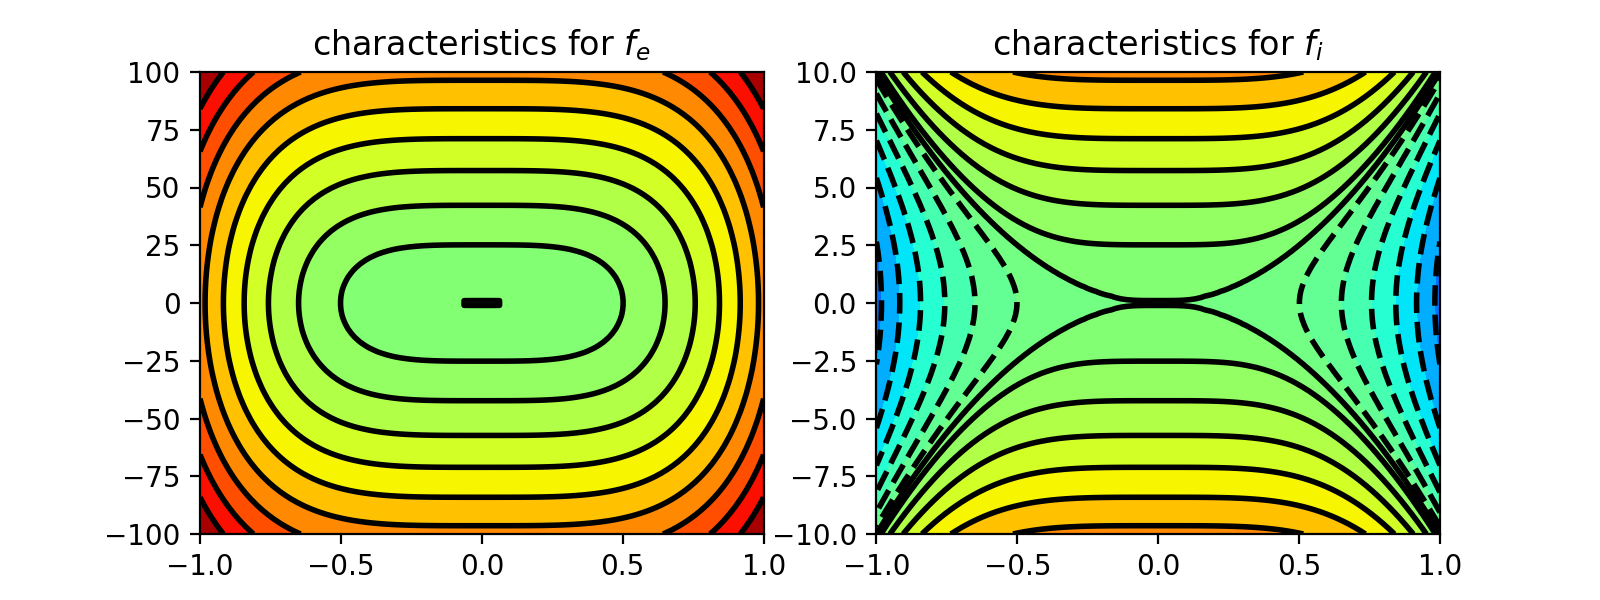
\includegraphics[width=0.9\linewidth]{images/characteristics}
%	\caption{Typical structure of the characteristic lines in the plan $(x,v)$.}
%	\label{fig:characteristics}
%\end{figure}
%
%Let us describe the fixed-point steps. Suppose that a candidate $\varphi^k$ is given. Then:
%\begin{enumerate}
%\item We may deduce the characteristic lines for the equations \cref{eq:sta_model_fi,eq:sta_model_fe}, and compute approximations $f_{i,e}^k$.
%\item By integration on $v$, we may compute $n^k \coloneqq n_i^k - n_e^k$.
%\item The next iterate $\varphi^{k+1}$ is defined as the solution of the Poisson problem \cref{eq:sta_model_phi} with source term $n^k$.
%\end{enumerate}

\section{Numerical results}
\subsection{1-species validation test case}
%\subsection{2-species results}
% Diagnostics (conservations)
% Do we observe sheaths? 
\subsection{Comparison between (SL) and (FD)}
%\subsection{Comparison between (SL) and (FP)}
%% plugging one into the other and the other way around

\bibliographystyle{alpha}
\bibliography{CEMRACS.bib}

\end{document}